%\section{従来の戦略の問題点}
%ここではベーシックストラテジーの問題点について述べる。ベーシックストラテジーの問題点はデック数が無限の場合を想定しており、既に引いたカードの種類や枚数が考慮されていない点である。

%基本的に実際に行われるゲームでは使用するデック数は有限である。デック数が有限であるということは、ゲーム中に使われたカードによって、次に引くカードの確率が変化していくということである。逆にデック数が無限であるということは、どのカードも常に一定の確率で引くということである。

%例えば図\ref{fig:deck}の場合を考える。デック数が1の場合は10のカードを引いたとき、$次に10のカードを引く確率は\frac{3}{51}となる。しかしデック数が無限の場合は次に10を引く確率は\frac{4}{52}となる。この部分がベーシックストラテジーと実際のゲームの違いである。ベーシックストラテジーではこの違いを考慮していないため実際ゲームの勝率とは差が出てしまう。$

%またベーシックストラテジーは勝率が4割程度しかなく、勝利数だけで言えばカジノ側に負けてしまうという問題点もある。カウンティングの問題点については後期に詳しく調査する予定である。

%\begin{figure}[H]
%\begin{center}
%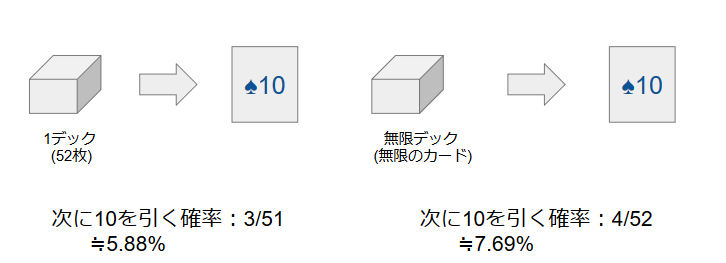
\includegraphics[width = 13cm]{./figure./DeckDiff.png}
%\caption{デック数による違い}
%\label{fig:deck}
%\end{center}
%\end{figure}

%\bunseki{※伊藤晋之介}

\section{戦略同士の比較}
Thorp氏によって考案されたベーシックストラテジーについて検証を行う。
ベーシックストラテジーの性能評価のために比較対象として6つの戦略を考えた。
比較対象となる戦略は次の通りである。

\begin{itemize}
  \item ベーシックストラテジー改変1
  \item ベーシックストラテジー改変2
  \item プレイヤーの合計値が15以上になるまでヒットする戦略
  \item プレイヤーの合計値が16以上になるまでヒットする戦略
  \item プレイヤーの合計値が17以上になるまでヒットする戦略
  \item プレイヤーの合計値が18以上になるまでヒットする戦略
\end{itemize}

以上の6つの戦略について、これから詳細に説明する。
\bunseki{※米村祥裕}

\subsection{ベーシックストラテジー改変1}
ベーシックストラテジーはブラックジャックにおける有効な戦略の一つである。しかし
戦略の表に注目すると、表の複雑性を考えたときに変更の余地があると考えた。
戦略表においてプレイヤーの合計値が12の行に注目する。ディーラーのアップカードが2、3の時は
Sとなっているが、その後アップカードが4、5、6の時はH、アップカードが7、8、9、10、Aの時はHとなっており、
Hに挟まれてSが存在している。表を覚えることを考えると、同じ行の中で変化が少ない方がよいと考えられる。
そのため、ベーシックストラテジー改変1では表\ref{bschange1}に示すようにプレイヤーの合計値が12、ディーラーのアップ
カードが4、5、6の時の戦略をSに変更した.
\bunseki{※米村祥裕}

\begin{table}[htbp]
  \centering
  \caption{ベーシックストラテジー改変1\label{bschange1}}
  \begin{tabular}{|c|c|c|c|c|c|c|c|c|c|c|c|}
    \hline
    \multicolumn{2}{|c|}{} & \multicolumn{10}{|c|}{ディーラーのアップカード} \\ \hline
    \multicolumn{2}{|c|}{} & 2 & 3 & 4 & 5 & 6 & 7 & 8 & 9 & 10 & A \\ \hline
    手札の合計 & 19以上 & S & S & S & S & S & S & S & S & S & S \\ \cline{3-12}
              & 18 & S & S & S & S & S & S & S & S & S & S \\ \cline{3-12}
              & 17 & S & S & S & S & S & S & S & S & S & S \\ \cline{3-12}
              & 16 & S & S & S & S & S & H & H & H & H & H \\ \cline{3-12}
              & 15 & S & S & S & S & S & H & H & H & H & H \\ \cline{3-12}
              & 13~14 & S & S & S & S & S & H & H & H & H & H \\ \cline{3-12}
              & 12 & S & S & S & S & S & H & H & H & H & H \\ \cline{3-12}
              & 11以下 & H & H & H & H & H & H & H & H & H & H \\ \hline
  \end{tabular}
\end{table}

\subsection{ベーシックストラテジー改変2}
ベーシックストラテジー改変1と同様にベーシックストラテジーの戦略表を改変した。
変更点はベーシックストラテジー改変1と同様にプレイヤーの合計値が12の行である。改変1ではディーラーのアップカードが4、5、6の部分を
Sに変更したが、改変2ではHに変更した。この変更によってプレイヤーの合計値が12の行はすべてHという表\ref{bschange2}ができた。
\bunseki{※米村祥裕}

\begin{table}[htbp]
  \centering
  \caption{ベーシックストラテジー改変2\label{bschange2}}
  \begin{tabular}{|c|c|c|c|c|c|c|c|c|c|c|c|}
    \hline
    \multicolumn{2}{|c|}{} & \multicolumn{10}{|c|}{ディーラーのアップカード} \\ \hline
    \multicolumn{2}{|c|}{} & 2 & 3 & 4 & 5 & 6 & 7 & 8 & 9 & 10 & A \\ \hline
    手札の合計 & 19以上 & S & S & S & S & S & S & S & S & S & S \\ \cline{3-12}
              & 18 & S & S & S & S & S & S & S & S & S & S \\ \cline{3-12}
              & 17 & S & S & S & S & S & S & S & S & S & S \\ \cline{3-12}
              & 16 & S & S & S & S & S & H & H & H & H & H \\ \cline{3-12}
              & 15 & S & S & S & S & S & H & H & H & H & H \\ \cline{3-12}
              & 13~14 & S & S & S & S & S & H & H & H & H & H \\ \cline{3-12}
              & 12 & H & H & H & H & H & H & H & H & H & H \\ \cline{3-12}
              & 11以下 & H & H & H & H & H & H & H & H & H & H \\ \hline
  \end{tabular}
\end{table}

\subsection{プレイヤーの合計値が一定以上になるまでヒットする戦略}
ディーラーがある程度有利な戦略を採用しているという仮定の下で、プレイヤーもディーラーと同様の
行動を行う戦略を考えた。プレイヤーの手札の合計値が一定以上になるまでヒットするものとして、次の4つの戦略を用意した。
\begin{itemize}
  \item プレイヤーの合計値が15以上になるまでヒットする戦略
  \item プレイヤーの合計値が16以上になるまでヒットする戦略
  \item プレイヤーの合計値が17以上になるまでヒットする戦略
  \item プレイヤーの合計値が18以上になるまでヒットする戦略
\end{itemize}
\bunseki{※米村祥裕}

\begin{table}[!hp]
  \centering
  \caption{プレイヤーの合計値が15以上になるまでヒットする戦略\label{hitleq15}}
  \begin{tabular}{|c|c|c|c|c|c|c|c|c|c|c|c|}
    \hline
    \multicolumn{2}{|c|}{} & \multicolumn{10}{|c|}{ディーラーのアップカード} \\ \hline
    \multicolumn{2}{|c|}{} & 2 & 3 & 4 & 5 & 6 & 7 & 8 & 9 & 10 & A \\ \hline
    手札の合計 & 19以上 & S & S & S & S & S & S & S & S & S & S \\ \cline{3-12}
              & 18 & S & S & S & S & S & S & S & S & S & S \\ \cline{3-12}
              & 17 & S & S & S & S & S & S & S & S & S & S \\ \cline{3-12}
              & 16 & S & S & S & S & S & S & S & S & S & S \\ \cline{3-12}
              & 15 & S & S & S & S & S & S & S & S & S & S \\ \cline{3-12}
              & 13~14 & H & H & H & H & H & H & H & H & H & H \\ \cline{3-12}
              & 12 & H & H & H & H & H & H & H & H & H & H \\ \cline{3-12}
              & 11以下 & H & H & H & H & H & H & H & H & H & H \\ \hline
  \end{tabular}
\end{table}

\begin{table}[p]
  \centering
  \caption{プレイヤーの合計値が16以上になるまでヒットする戦略\label{hitleq16}}
  \begin{tabular}{|c|c|c|c|c|c|c|c|c|c|c|c|}
    \hline
    \multicolumn{2}{|c|}{} & \multicolumn{10}{|c|}{ディーラーのアップカード} \\ \hline
    \multicolumn{2}{|c|}{} & 2 & 3 & 4 & 5 & 6 & 7 & 8 & 9 & 10 & A \\ \hline
    手札の合計 & 19以上 & S & S & S & S & S & S & S & S & S & S \\ \cline{3-12}
              & 18 & S & S & S & S & S & S & S & S & S & S \\ \cline{3-12}
              & 17 & S & S & S & S & S & S & S & S & S & S \\ \cline{3-12}
              & 16 & S & S & S & S & S & S & S & S & S & S \\ \cline{3-12}
              & 15 & H & H & H & H & H & H & H & H & H & H \\ \cline{3-12}
              & 13~14 & H & H & H & H & H & H & H & H & H & H \\ \cline{3-12}
              & 12 & H & H & H & H & H & H & H & H & H & H \\ \cline{3-12}
              & 11以下 & H & H & H & H & H & H & H & H & H & H \\ \hline
  \end{tabular}
\end{table}

\begin{table}[p]
  \centering
  \caption{プレイヤーの合計値が17以上になるまでヒットする戦略\label{hitleq17}}
  \begin{tabular}{|c|c|c|c|c|c|c|c|c|c|c|c|}
    \hline
    \multicolumn{2}{|c|}{} & \multicolumn{10}{|c|}{ディーラーのアップカード} \\ \hline
    \multicolumn{2}{|c|}{} & 2 & 3 & 4 & 5 & 6 & 7 & 8 & 9 & 10 & A \\ \hline
    手札の合計 & 19以上 & S & S & S & S & S & S & S & S & S & S \\ \cline{3-12}
              & 18 & S & S & S & S & S & S & S & S & S & S \\ \cline{3-12}
              & 17 & S & S & S & S & S & S & S & S & S & S \\ \cline{3-12}
              & 16 & H & H & H & H & H & H & H & H & H & H \\ \cline{3-12}
              & 15 & H & H & H & H & H & H & H & H & H & H \\ \cline{3-12}
              & 13~14 & H & H & H & H & H & H & H & H & H & H \\ \cline{3-12}
              & 12 & H & H & H & H & H & H & H & H & H & H \\ \cline{3-12}
              & 11以下 & H & H & H & H & H & H & H & H & H & H \\ \hline
  \end{tabular}
\end{table}

\begin{table}[p]
  \centering
  \caption{プレイヤーの合計値が18以上になるまでヒットする戦略\label{hitleq18}}
  \begin{tabular}{|c|c|c|c|c|c|c|c|c|c|c|c|}
    \hline
    \multicolumn{2}{|c|}{} & \multicolumn{10}{|c|}{ディーラーのアップカード} \\ \hline
    \multicolumn{2}{|c|}{} & 2 & 3 & 4 & 5 & 6 & 7 & 8 & 9 & 10 & A \\ \hline
    手札の合計 & 19以上 & S & S & S & S & S & S & S & S & S & S \\ \cline{3-12}
              & 18 & S & S & S & S & S & S & S & S & S & S \\ \cline{3-12}
              & 17 & H & H & H & H & H & H & H & H & H & H \\ \cline{3-12}
              & 16 & H & H & H & H & H & H & H & H & H & H \\ \cline{3-12}
              & 15 & H & H & H & H & H & H & H & H & H & H \\ \cline{3-12}
              & 13~14 & H & H & H & H & H & H & H & H & H & H \\ \cline{3-12}
              & 12 & H & H & H & H & H & H & H & H & H & H \\ \cline{3-12}
              & 11以下 & H & H & H & H & H & H & H & H & H & H \\ \hline
  \end{tabular}
\end{table}
\newpage

\subsection{複雑性の定義について}

プレイヤーに扱いやすい戦略とは何かを定義する為に、戦略の複雑性を次のように定義した。
まず、戦略の文字列を圧縮する。元の表を「連続する文字+連続して文字が出た回数」と変換することで文字列を圧縮した。
例として、「HHSSSHHHHH」という10文字からなる文字列を圧縮すると、「H2S3H5」となり、圧縮した後の文字列は6文字
となる。また「HHHHHHHHHH」という文字列を「H10」と圧縮したときのように、連続して同じ文字が出た回数が2桁の場合には
数字部分を1文字として数える。つまり「H10」の文字列長は2文字である。

圧縮した後の文字列長を元の表の大きさ(80)で割った数値を複雑性の定義とした。
\bunseki{※米村祥裕}

\subsection{各戦略の複雑性}

%用意した戦略は次のような8行の配列とし、それぞれの行に圧縮を行った。\\

%\begin{table}[H]
%\caption{ベーシックストラテジーの戦略表}
%\label{table:data_type}
%\begin{center}
%\begin{tabular}{|cc|c|c|c|c|c|c|c|c|c|c|}
%\hline
%                            &            & \multicolumn{10}{c|}{ディーラーのアップカード}     \\ \cline{3-12} 
%                            &            & 2 & 3 & 4 & 5 & 6 & 7 & 8 & 9 & 10 & A \\ \hline
%\multicolumn{1}{|l|}{手札の合計} & 19以上       & S & S & S & S & S & S & S & S & S  & S \\ \cline{2-12} 
%\multicolumn{1}{|l|}{}      & 18         & S & S & S & S & S & S & S & S & S  & S \\ \cline{2-12} 
%\multicolumn{1}{|l|}{}      & 17         & S & S & S & S & S & S & S & S & S  & S \\ \cline{2-12} 
%\multicolumn{1}{|l|}{}      & 16         & S & S & S & S & S & H & H & H & H  & H \\ \cline{2-12} 
%\multicolumn{1}{|l|}{}      & 15         & S & S & S & S & S & H & H & H & H  & H \\ \cline{2-12} 
%\multicolumn{1}{|l|}{}      & 13$\sim$14 & S & S & S & S & S & H & H & H & H  & H \\ \cline{2-12} 
%\multicolumn{1}{|l|}{}      & 12         & H & H & S & S & S & H & H & H & H  & H \\ \cline{2-12} 
%\multicolumn{1}{|l|}{}      & 11以下       & H & H & H & H & H & H & H & H & H  & H \\ \hline
%\end{tabular}
%\end{center}
%\end{table}

今回用意した戦略を、全て圧縮したのが表\ref{table:data_type}である。


%\begin{figure}[htbp]
%\begin{center}
%\includegraphics[width=15cm,bb=0 0 602 261]{2.png}
%\end{center}
%\caption{各戦略の圧縮した後の文字列と複雑性}
%\label{picture}
%\end{figure}

\begin{table}[H]
\caption{各戦略の圧縮した後の文字列と複雑性\label{table:data_type}}
\begin{center}
\begin{tabular}{|c|c|c|c|}
\hline
戦略           & 圧縮した後の文字列                                                                   & 文字列長 & 複雑性   \\ \hline
ベーシックストラテジー         & \begin{tabular}[c]{@{}l@{}}S10S5H5S5H5S5H5S5H5S5H5H2S3H5H10\end{tabular} & 30   & 0.375 \\ \hline
ベーシックストラテジー改変1      & S10S5H5S5H5S5H5S5H5S5H5S5H5H10                                              & 28   & 0.35  \\ \hline
ベーシックストラテジー改変2      & S10S5H5S5H5S5H5S5H5S5H5H10H10                                               & 26   & 0.325 \\ \hline
15以上になるまでヒットする戦略 & S10S10S10S10S10H10H10H10                                                    & 16   & 0.2   \\ \hline
16以上になるまでヒットする戦略 & S10S10S10S10H10H10H10H10                                                    & 16   & 0.2   \\ \hline
17以上になるまでヒットする戦略 & S10S10S10H10H10H10H10H10                                                    & 16   & 0.2   \\ \hline
18以上になるまでヒットする戦略 & S10S10H10H10H10H10H10H10                                                    & 16   & 0.2   \\ \hline
\end{tabular}
\end{center}
\end{table}

表\ref{table:data_type}を見ると、ベーシックストラテジーを改変した戦略の方が、複雑性が低く、プレイヤーにとって扱いやすいといえる。
また、手札の合計値が一定以上になるまでヒットする戦略は、複雑性がベーシックストラテジーの半分程度であり、プレイヤーに
とって扱いやすい戦略だといえる。
\bunseki{※渡邊凛}

